
\section{Querying over multiple tables $\to$ Joins}

%------------------------------------------------------------------------------
\begin{frame}[fragile, allowframebreaks]{SQL as a query language: \texttt{JOINS}}
\metroset{block=fill}
\footnotesize
In the \texttt{CREATE} command, we defined a table and set up a relational database using keys (SQL's data definition language). Now we want to analyze (i.e. query) our database to learn about the contents.

\begin{block}{Remember: Foreign Keys}\footnotesize
Foreign keys (\emph{Fremdschlüssel}) are table cells containing ID number which uniquely reference the primary keys (\emph{Primärschlüssel}) of another table.

For example the table \texttt{books} contains a column \texttt{publisher\_id} which references one particular entry of the table \texttt{publishers} via its \texttt{publisher\_id}.

\begin{sqlcode}
    SELECT title, publisher_id FROM books ;
\end{sqlcode}

\footnotesize
\textbf{Attention:} The table columns you link up don't necessarily share the same name (unless you made it so!) 

\textbf{Attention:} Because foreign keys don't have to be unique they're no true keys -- they are still named that way. 
\end{block}

\framebreak
\begin{block}{Linking tables in queries}\small 
If you link up the table \texttt{books} to the table \texttt{publishers} using the \texttt{books}' tables foreign key \texttt{publisher\_id}, you get a new relation containg all contents of both tables.
\begin{sqlcode}
SELECT *
FROM books, publishers
WHERE books.publisher_id = publishers.publisher_id ;
\end{sqlcode}

\centering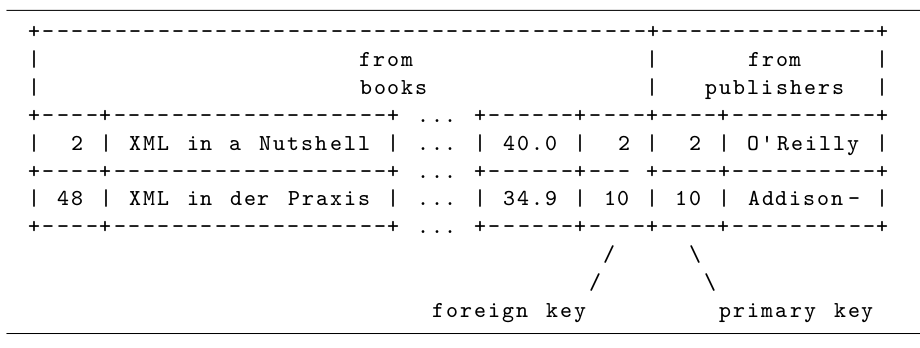
\includegraphics[width=0.7\textwidth]{img/foreign-keys.png}
\medskip

\end{block}


\framebreak

\begin{columns}
\column{0.48\textwidth}
  \begin{block}{Table-specific columns I}\scriptsize
In case we're only interested in specific columns of the linked tables, we can pick just those in the 
 \texttt{SELECT} statement. Be mindful of potential name conflicts due to ambiguous column names. 
In those cases, you need to specifically adress them like so: 
\begin{sqlcode}
SELECT title, publisher_name, 
  books.publisher_id,
  publishers.publisher_id
FROM books, publishers
WHERE books.publisher_id 
  = publishers.publisher_id;
\end{sqlcode}
\end{block}

\column{0.49\textwidth}
\begin{block}{Table-specific columns  II}\scriptsize
Because the column name \texttt{publisher\_id} exists both in \texttt{books} as well as in  \texttt{publishers} we need to tell the DBMS which one we mean by prefacing it with its parent table: 
\texttt{books.publisher\_id}.

In longer queries it cam make sense to abbreviate table names to save some typing and keep a better overview: 

\begin{sqlcode}
SELECT title, publisher_name, 
   b.publisher_id, 
   p.publisher_id
FROM books b, publishers p
WHERE b.publisher_id 
   = p.publisher_id;
\end{sqlcode}
\end{block}
\end{columns}

\framebreak

\begin{block}{Attention: Avoid the cartesian product!}\footnotesize
When joining multiple tables, it is essential that you specify conditions for it: 

\begin{sqlcode}
SELECT count(*) FROM books ;
SELECT count(*) FROM publishers ;
SELECT count(*) FROM books, publishers ;
SELECT count(*) FROM books, publishers
WHERE books.publisher_id = publishers.publisher_id ;
\end{sqlcode}
These queries give the following result counts: 353, 82, 28946, 350.

The number of result lines in joins equals the product of the lines of all the joined tables. That way, we can easily generate results with millions (!) of  lines which excede your database servers capacity and thus, might crash it. 

Thus: 
\alert{Careful not to accidentally produce the cartesian product of multiple columns!}

\end{block}
\end{frame}

%------------------------------------------------------------------------------
\begin{frame}[fragile, allowframebreaks]{JOINs}
\metroset{block=fill}

\begin{columns}
\column{0.48\textwidth}
\begin{block}{Linking tables using \texttt{WHERE}}\small
The \texttt{WHERE} clause compares if values from one table are present in another table: 
\begin{sqlcode}
SELECT tab1.* FROM tab1, tab2 
WHERE tab1.tab2_fk = tab2.id ; 
\end{sqlcode}
\end{block}

\column{0.48\textwidth}
\begin{block}{Linking tables using \texttt{JOIN}}\footnotesize
In the \texttt{FROM} clause, tables are linked using the \texttt{JOIN} statement:
\begin{sqlcode}
SELECT tab1.* FROM tab1 
JOIN tab2 
ON tab1.tab2_fk = tab2.id; 
\end{sqlcode}

This syntax allows us to decide what happens if one of the tables contains no relevant values (e.g. `Give me the names of all course participants and their Bachelor field of origin, in case they already have a Bachelor's degree.').
\end{block}
\end{columns}

\framebreak

\small
Show me the distance to each of the lakes in the database from the hotel with the name „Schlossberghotel“:
\begin{sqlcode}
SELECT see.name, strasse.distanz 
FROM strasse, see, hotel 
WHERE hotel.name = 'Schlossberghotel' 
    AND strasse.hotel_fk = hotel.hotel_id 
    AND strasse.see_fk = see.see_id ;
\end{sqlcode}

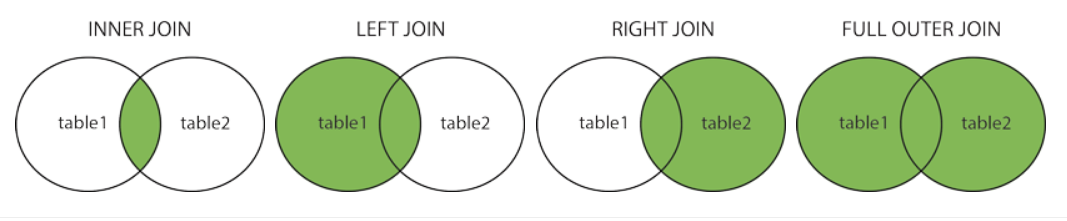
\includegraphics[width=\textwidth]{img/sql-joins-w3.png}
{\scriptsize
Source: \href{https://www.w3schools.com/sql/sql_join.asp}{W3Schools Joins}
}

\framebreak


\begin{block}{JOINs}\small
Linking tables using conditions is called `joining them'. 
Joins are so common in database applicatoins that they have their own keyword in SQL: 
 \texttt{JOIN}.

The example from before:
\begin{sqlcode}
SELECT title, publisher_name
FROM books, publishers
WHERE books.publisher_id = publishers.publisher_id ;
\end{sqlcode}
\dots can also be written like this:
\begin{sqlcode}
SELECT title, publisher_name
FROM books JOIN publishers
ON books.publisher_id = publishers.publisher_id ;
\end{sqlcode}
\end{block}


\framebreak
\begin{block}{\texttt{JOIN and USING}}\small
If both tables linked by the join \texttt{JOIN} share the same names, you can shorten the command like so: 
\begin{sqlcode}
SELECT title, publisher_name
FROM books JOIN publishers USING ( publisher_id );
\end{sqlcode}
\end{block}

\begin{block}{NATURAL JOIN I}\footnotesize
If two tables share the same column names, one can use \texttt{NATURAL JOIN} to link them. Be careful -- the DBMS will try to use \emph{all} common column names for the comparison!
\begin{sqlcode}
SELECT title, publisher_name
FROM books NATURAL JOIN publishers ;
\end{sqlcode}

\end{block}

\framebreak

\begin{block}{NATURAL JOIN II}\footnotesize
Will give the same result as the last query. However, a \texttt{NATURAL
JOIN} will compare \textbf{all} columns sharing the same name in both tables. 
If, for example, the table \texttt{publishers} had another column called \texttt{title}, the \texttt{NATURAL JOIN} would deliver an empty result because the query would correspond to this:
\begin{sqlcode}
SELECT title, publisher_name
FROM books, publishers
WHERE books.publisher_id = publishers.publisher_id
AND books.title = publishers.title ;
\end{sqlcode}

The DMBS will try to link \textbf{all} columns with the same name in a \texttt{NATURAL JOIN}!
\end{block}

\framebreak

\begin{block}{JOINS over multiple tables}\small
In practice you often need to link more than two tables to achieve the desired result. That's why 
\texttt{JOIN} can be used as many times as needed per query: 
\begin{sqlcode}
SELECT title, publisher_name, binding
FROM books
JOIN publishers USING ( publisher_id )
JOIN bindings ON books.binding_id = bindings.id ;
\end{sqlcode}
\end{block}

\framebreak

\begin{block}{JOINs for n:m relationships}\small
Tables used n:m relationships function the same way as all others. To query all authors of a book, you would use the following command:  
\begin{sqlcode}
SELECT books.title , authors.firstname , authors.lastname
FROM books
JOIN authors_books USING ( book_id )
JOIN authors USING ( author_id ) ;
\end{sqlcode}
Each combination will be outputted in a single line. Thus, if a book has three authors, for example, you would get three a three-line result. 
\end{block}

\framebreak 

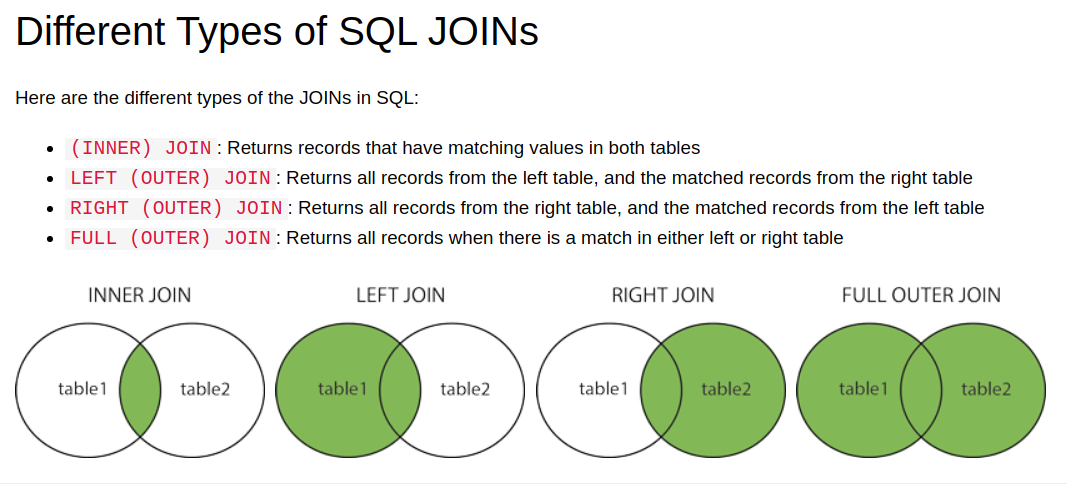
\includegraphics[width=\textwidth]{img/w3schools-joins.png}
{\scriptsize
Source: \href{https://www.w3schools.com/sql/sql_join.asp}{W3Schools Joins}
}

\framebreak

\begin{block}{INNER JOIN}\footnotesize
Until now, we have been using \texttt{JOIN} to link tables. However, strictly speaking, these were all  \texttt{INNER JOIN}s. Because \texttt{INNER JOIN}s are so frequent, you can use the shorthand \texttt{JOIN}  instead of the long form.

But if there is an \texttt{INNER JOIN}, there must be an \texttt{OUTER JOIN} as well.
The difference is in the way it handles missing values: An \texttt{INNER JOIN} would display nothing if there is no value corresponding to the foreign key, whereas the \texttt{OUTER JOIN} would.

Let's check if there are books with no publisher:
\begin{sqlcode}
SELECT book_id, title FROM books WHERE publisher_id IS NULL ;
\end{sqlcode}
\end{block}

\framebreak 

\begin{block}{INNER versus OUTER JOIN: INNER}\footnotesize
What happens in an \texttt{INNER JOIN} when we come across a book without a value for the \texttt{publisher} field?

\begin{sqlcode}
SELECT books.title, publishers.publisher_name
FROM books
INNER JOIN publishers USING ( publisher_id )
WHERE books.book_id IN (3199, 3209, 3210) ;
\end{sqlcode}

Since there is no corresponding entry in \texttt{publishers} the data from \texttt{books} isn't printed either.
\end{block}

\framebreak 



\begin{columns}
\column{0.48\textwidth}
\begin{block}{(INNER) JOIN}\small
Only data points having a correspondent on both sides are printed: 

\begin{sqlcode}
SELECT studis.name, titel.abk 
FROM studis 
JOIN titel 
ON studis.titel = titel.abk ;
\end{sqlcode}
\end{block}

\column{0.48\textwidth}
\begin{block}{LEFT JOIN}\small
All entries in the table before \texttt{LEFT JOIN} are printed and the ones from the one on the right only if they correspond to the \texttt{ON} clause.

\begin{sqlcode}
SELECT studis.name, titel.abk 
FROM studis 
LEFT JOIN titel 
ON studis.titel = titel.abk ;
\end{sqlcode}
\end{block}
\end{columns}


\begin{sqlcode}
SELECT distanz, see.name, hotel.name 
FROM strasse 
INNER JOIN see ON see.see_id = strasse.see_fk 
INNER JOIN hotel 
ON hotel.hotel_id = strasse.hotel_fk;
\end{sqlcode}


\begin{columns}
\column{0.3\textwidth}
\begin{block}{JOIN (FROM)}\footnotesize
Querying entities or relationships (entries from multiple tables) which are connected using foreign keys. 
\end{block}

\column{0.3\textwidth}
\begin{block}{INNER JOIN}\footnotesize
Indicates which tables (or their entries) are linked up, i.e. represented in a new view together. 

\end{block}

\column{0.3\textwidth}
\begin{block}{ON}\footnotesize
Defines the criterion on which to perform the join.
\end{block}
\end{columns}

\framebreak 

\begin{block}{INNER versus OUTER JOIN: OUTER}\footnotesize
In an \texttt{OUTER JOIN} the search result looks like the following:
\begin{sqlcode}
SELECT books.title, publishers.publisher_name
FROM books
LEFT OUTER JOIN publishers USING ( publisher_id )
WHERE books.book_id IN (3199, 3209, 3210) ;
\end{sqlcode}
\centering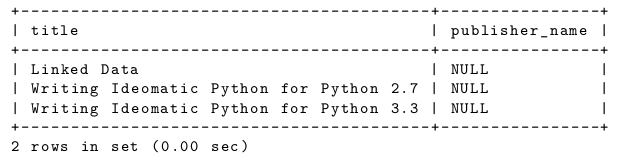
\includegraphics[width=0.7\textwidth]{img/outer-join-null.png}
\medskip
\end{block}
\footnotesize
These are the three entries from earlier which were missing in our first \texttt{COUNT(*)} example: \texttt{books} contains 353 entries but the \texttt{JOIN} only resulted in 350 because these three entries have missing values in the \texttt{publisher} field. 

\framebreak 

\begin{block}{LEFT OUTER JOIN}\small
\texttt{OUTER JOIN} can't be used on it's own. You need to specify the directionality, indicating in which table values can be missing.
\begin{sqlcode}
SELECT books.title, publishers.publisher_name
FROM books
RIGHT OUTER JOIN publishers USING ( publisher_id )
WHERE books.book_id IN (3199, 3209, 3210) ;
\end{sqlcode}

\begin{verbatim}
    Empty set (0.00 sec )
\end{verbatim}
\end{block}

\framebreak 

\begin{block}{RIGHT OUTER JOIN}\small
If we invert the order of the tables in the query, the \texttt{RIGHT OUTER JOIN} works:
\begin{sqlcode}
SELECT books.title, publishers.publisher_name
FROM publishers
RIGHT OUTER JOIN books USING ( publisher_id )
WHERE books.book_id IN (3199, 3209, 3210) ;
\end{sqlcode}
\end{block}

\framebreak

\begin{block}{FULL (OUTER) JOIN}\small
\texttt{FULL OUTER JOIN} is equivalent to \texttt{FULL JOIN}. It will give you all entries of the database, irrespective of missing values. Be careful, the result may be large! 
\begin{sqlcode}
SELECT column_name(s)
FROM table1
FULL OUTER JOIN table2
ON table1.column_name = table2.column_name
WHERE condition;
\end{sqlcode}
\end{block}

By comparison, the \texttt{INNER JOIN} that is our most common, go-to normal \texttt{JOIN} will handle missing values very differently: It will only print complete records! If one value is missing, the whole record will not be printed, so make sure to use \texttt{COUNT(*)} for the result of different types of joins (full outer or normal inner join) to check if the numbers differs!

\end{frame}

 

%TODO
\section{Exercise using \texttt{urlaub.db}}

%------------------------------------------------------------------------------
\begin{frame}[fragile]{Exercise using \texttt{urlaub.db}}
\metroset{block=fill}
\begin{columns}
  \column{0.65\textwidth}
      \begin{exampleblock}{Exercise: Overview over the DB}\footnotesize
Open the example database \texttt{urlaub.db} and construct SQL queries for the following tasks: 
        \begin{enumerate}\scriptsize
    \item You want to get an overview of the attributes of the lakes in the table \texttt{see}. Look up the structure of the table using \texttt{.schema} and then, query all information contained in the table for maximum two lakes.  
    \item You're interested mainly in the names and depths of the lakes. Query just those two attributes!
    \item You're scared of lakes deeper than 10 meters, thus, query only those which aren't deeper than 10m. 
\end{enumerate}
      \end{exampleblock}
  \column{0.35\textwidth}
    \begin{block}{Getting an overview}\small
    First find out which info (table names) the database even contains using \texttt{.schema}, then try\dots
    \begin{sqlcode}
    SELECT * FROM table; 
    etc.
    \end{sqlcode}
\end{block}

\end{columns}
\end{frame}


%------------------------------------------------------------------------------
\begin{frame}[fragile]{Exercise using \texttt{urlaub.db}}
\metroset{block=fill}
  \begin{columns}[T,onlytextwidth]
    \column{0.35\textwidth}
      \begin{exampleblock}{Exercise 1 continued\dots}\footnotesize
You like your creature comforts but would like to save money still. Thus, query the names and hotel IDs for all the hotels which have more than three stars (\texttt{austattung}) and are priced below 100€.
      \end{exampleblock}


    \column{0.6\textwidth}
      \begin{alertblock}{Advanced: Linking tables}\scriptsize
      \begin{enumerate}
          \item You want the hotels and lakes which fit your requirements \emph{and} are connected by a road. First, find out which hotels and lakes are connected by a direct path by inspecting the \texttt{straße} table and including \textbf{hotel} and \texttt{see} using a join.
          \item Only query the connecting roads for hotels and lakes which meet your requirements and count the number of results. 
          \item Your ideal lake-hotel combination is the one where the length of the road/connection is as short as possible: Sort the result in ascending order highlighting the shortest distance. \\
          \item Find out the average price of hotels per star rating. \\
          \item \textbf{Bonus:} What is the name of the place in which the hotel with the shortest distance to your preferred lake is located? 
      \end{enumerate}
      \end{alertblock}

  \end{columns}
\end{frame}

%------------------------------------------------------------------------------
%\begin{frame}[standout]\alert{Hausübung:} \end{frame}
%TODO already appeared in the SQL.tex slides

\section{Sample solution for the \texttt{urlaub.db} exercise}
%------------------------------------------------------------------------------
\begin{frame}[allowframebreaks, fragile]{Sample solution for the \texttt{urlaub.db} exercise}
\scriptsize

\begin{columns}
  \column{0.45\textwidth}
  At first, we need to find out which tables even exist in the database (what are their names so we can use the \texttt{.schema} command on them): What is the structure of the \texttt{see} table?
\begin{sqlcode}
    .tables
    SELECT * FROM see; 
    .schema see
    .mode column
\end{sqlcode}

Only show two results (as a preview): 
\begin{sqlcode}
    SELECT * FROM see
    LIMIT 2;
\end{sqlcode}

  \column{0.55\textwidth}
  
There is a column \verb|tiefe_in_m|:
\begin{sqlcode}
    SELECT name, tiefe_in_m FROM see;
\end{sqlcode}
Now we want to select lakes whose depth is smaller than 10m:

\begin{sqlcode}
    SELECT name, tiefe_in_m FROM see
    WHERE tiefe_in_m < 10;
\end{sqlcode}
\end{columns}

\framebreak 


\begin{columns}
  \column{0.35\textwidth}
  Concerning the hotels:
\begin{sqlcode}
    .tables
    SELECT * FROM hotel; 
    .schema hotel
\end{sqlcode} 
  \column{0.65\textwidth}
 
Show only \texttt{name} and \texttt{hotel\_id} for hotels with more than 3 stars which are under 100€:
\begin{sqlcode}
    SELECT name, hotel_id FROM hotel
    WHERE zimmerpreis < 100
    AND ausstattung >= 3;
\end{sqlcode}
For each of these examples, reflect whether you mean `equals' or `>=/<='.

Do we need to use parentheses so the query works?

Hint: It's usually more of a big deal with \texttt{OR}\dots
\end{columns}


\framebreak 

Find all hotels and lakes conected by a road: 

\begin{sqlcode}
SELECT see.name, strasse.distanz, hotel.name  
FROM strasse, see, hotel 
WHERE strasse.hotel_fk = hotel.hotel_id 
    AND strasse.see_fk = see.see_id ;
\end{sqlcode}

Or using \texttt{INNER JOIN}:
\begin{sqlcode}
SELECT distanz, see.name, hotel.name 
FROM strasse
INNER JOIN see ON see.see_id = strasse.see_fk
INNER JOIN hotel 
ON hotel.hotel_id = strasse.hotel_fk;
\end{sqlcode}

\framebreak 

Only show those which meet the criteria we defined earlier:
\begin{sqlcode}
SELECT see.name, strasse.distanz, hotel.name  
FROM strasse, see, hotel 
WHERE strasse.hotel_fk = hotel.hotel_id 
    AND strasse.see_fk = see.see_id 
    AND see.tiefe_in_m < 10
    AND (hotel.zimmerpreis < 100 AND hotel.ausstattung >= 3);
\end{sqlcode}

Now we want to sort by minimum distance, showing the results in ascending order so that the shortest distance comes first. Modify the previous query by adding this at the end:
\begin{sqlcode}
ORDER BY strasse.distanz ASC;
\end{sqlcode}

\framebreak 


\begin{columns}
\medskip

  \column{0.57\textwidth}
  Average price of the hotels:
\begin{sqlcode}
SELECT AVG(zimmerpreis) FROM hotel;
\end{sqlcode}
Or for all with less than 3 stars:
\begin{sqlcode}
SELECT AVG(zimmerpreis) FROM hotel
WHERE ausstattung < 3;
\end{sqlcode}

  \column{0.42\textwidth}
For hotels with 5 stars:
\begin{sqlcode}
SELECT AVG(zimmerpreis) 
FROM hotel
WHERE ausstattung = 5;
\end{sqlcode}
\end{columns}
\medskip

Where is the hotel with the shortest distance to the lake corresponding to your criteria?
\begin{sqlcode}
SELECT hotel.ort_id ort, hotel.name, 
       see.name, MIN(strasse.distanz)
FROM strasse, see, hotel 
WHERE see.tiefe_in_m < 10  AND strasse.see_fk = see.see_id 
    AND strasse.hotel_fk = hotel.hotel_id 
    AND (hotel.zimmerpreis < 100 AND hotel.ausstattung >= 3);
\end{sqlcode}
\end{frame}




\section{SQL addenda (auxiliary tables)}
%------------------------------------------------------------------------------
\begin{frame}[allowframebreaks, fragile]{Adding multiple values using auxiliary tables}
\footnotesize

\href{https://stackoverflow.com/questions/13487671/add-multiple-values-in-one-column}{Example for the use of auxiliary tables (from StackOverflow)}

\begin{columns}
  \column{0.35\textwidth}
  \begin{itemize}
      \item Each cell in a SQL table can only have one value. 
      \item \alert{Problem:} Some cells should actually be able to have more than one value.
      \item \alert{Solution:} Use auxiliary tables.
  \end{itemize}
   \column{0.65\textwidth}
\begin{sqlcode}
CREATE TABLE Product (
  ProductID INTEGER PRIMARY KEY,
  ProductName TEXT UNIQUE
);

CREATE TABLE Category (
  CategoryID INTEGER PRIMARY KEY,
  CategoryName TEXT UNIQUE
);

CREATE TABLE Product_Category (
  RecordID INT AUTO_INCREMENT PRIMARY KEY,
  CategoryID INT,
  ProductID INT
);
\end{sqlcode}
\end{columns}

\framebreak 

Example data record for the table:
\begin{sqlcode}
INSERT INTO Category VALUES (1, 'Fruit');
INSERT INTO Category VALUES (2, 'Vegetable');

INSERT INTO Product 
VALUES (1, 'Apple'),
       (2, 'Banana'), 
       (3, 'Cabbage'),
       (4, 'Squash'),
       (5, 'Tomato');

INSERT INTO Product_Category (CategoryID, ProductID) 
VALUES (1,1), (1,2), (2,3), (2,4), (1,5), (2,5);
\end{sqlcode}
%\href{http://sqlfiddle.com/#!2/fd0e2/3}{SQL-Fiddle Demo of this table}

\end{frame}



\section{SQL addenda (special queries)}
%------------------------------------------------------------------------------
\begin{frame}[allowframebreaks, fragile]{Querying multiple values}
\footnotesize

\begin{columns}
  \column{0.35\textwidth}
  \begin{itemize}
      \item In a common query, I can only query once from each table.
      \item \alert{Problem:} Assuming I want to query sender and recipient which are listed in the \texttt{Briefe} table with Foreign Key but both come from the \texttt{Personen} table.
      \item this db setup makes sense to avoid redundant data, so it's a legitimate problem you might encounter.
      \item \alert{Solution:} Include a subquery (cf. \href{https://stackoverflow.com/questions/41450663/selecting-same-column-twice-from-a-single-table-but-with-different-conditions}{StackOverflow}).
  \end{itemize}
   \column{0.65\textwidth}
\begin{sqlcode}
SELECT
    e.ID, 
    e.Name, 
    e.Boss, 
    (SELECT Name FROM Employees b 
     WHERE b.ID = e.Boss) as BossName
FROM Employees e;
\end{sqlcode}
Example by a previous student:
\begin{sqlcode}
SELECT l.Signatur_FK as Signatur, 
 (SELECT AutorName FROM Personen a 
  WHERE a.ID_Person = l.ID_Empfaenger_FK)
  as Empfaenger,  
 (SELECT AutorName FROM Personen b 
  WHERE b.ID_Person = l.ID_Absender_FK)
  as Absender 
FROM Abse_Empf l; /* l for the list */
\end{sqlcode}

\end{columns}

\end{frame}






